\documentclass[]{auvsi_doc}
\setkeys{auvsi_doc.cls}{
	AUVSITitle={Unmanned Ground Vehicle Delivery System Selected Concept Description},
	AUVSILogoPath={./figs/logo.pdf},
}

% include extra packages, if needed

% Remove Heading Numbers
\setcounter{secnumdepth}{0}

% Remove Heading Numbers
\setcounter{secnumdepth}{0}


% include extra packages, if needed

\begin{document}

\begin{AUVSITitlePage}
\begin{artifacttable}
\entry{GV-005, 1.0, 10-30-2018, Wrote concept description, Kameron Eves, Andrew Torgesen}
\entry{GV-005, 1.0, 2-21-2019, Updated to reflect subsystem engineering, Jacob Willis, Needs Checked}
% additional \entry{} commands for extra rows in the revision table, if needed
\end{artifacttable}
\end{AUVSITitlePage}

% document contents (see below for LaTex commands that make your life easier)
\section{Introduction}
This document gives a more detailed description of the selected concept for the UGV delivery system. The concept selected during concept development was a parachute with fins. After considering the added complexity of fins, and the small benefit they provide, we determined to simply use a parachute.

\section{Description}

The UGV will be loaded within the aircraft.
Upon a command from the flight controller system, a small hatch will open and the UGV will fall out. 
The UGV is carried to the ground by a lightweight 36 inch nylon parachute, purchased from FruityChutes. 
The parachute is loaded onto the aircraft in a tube that allows the UGV to pull it out of the aircraft as it falls. This helps stop the tangling that can come from a folded parachute. To also prevent tangling, and to make for a more predictable drop, the parachute is folding according to GV-007. After exiting the aircraft the parachute will be opened by drag. The drag caused by the fabric will slow down the system enough to allow the UGV to survive impact without damage. A visual depiction of our chosen system can be seen in Fig.~\ref{fig:side}.

\begin{figure}[h]
\centering
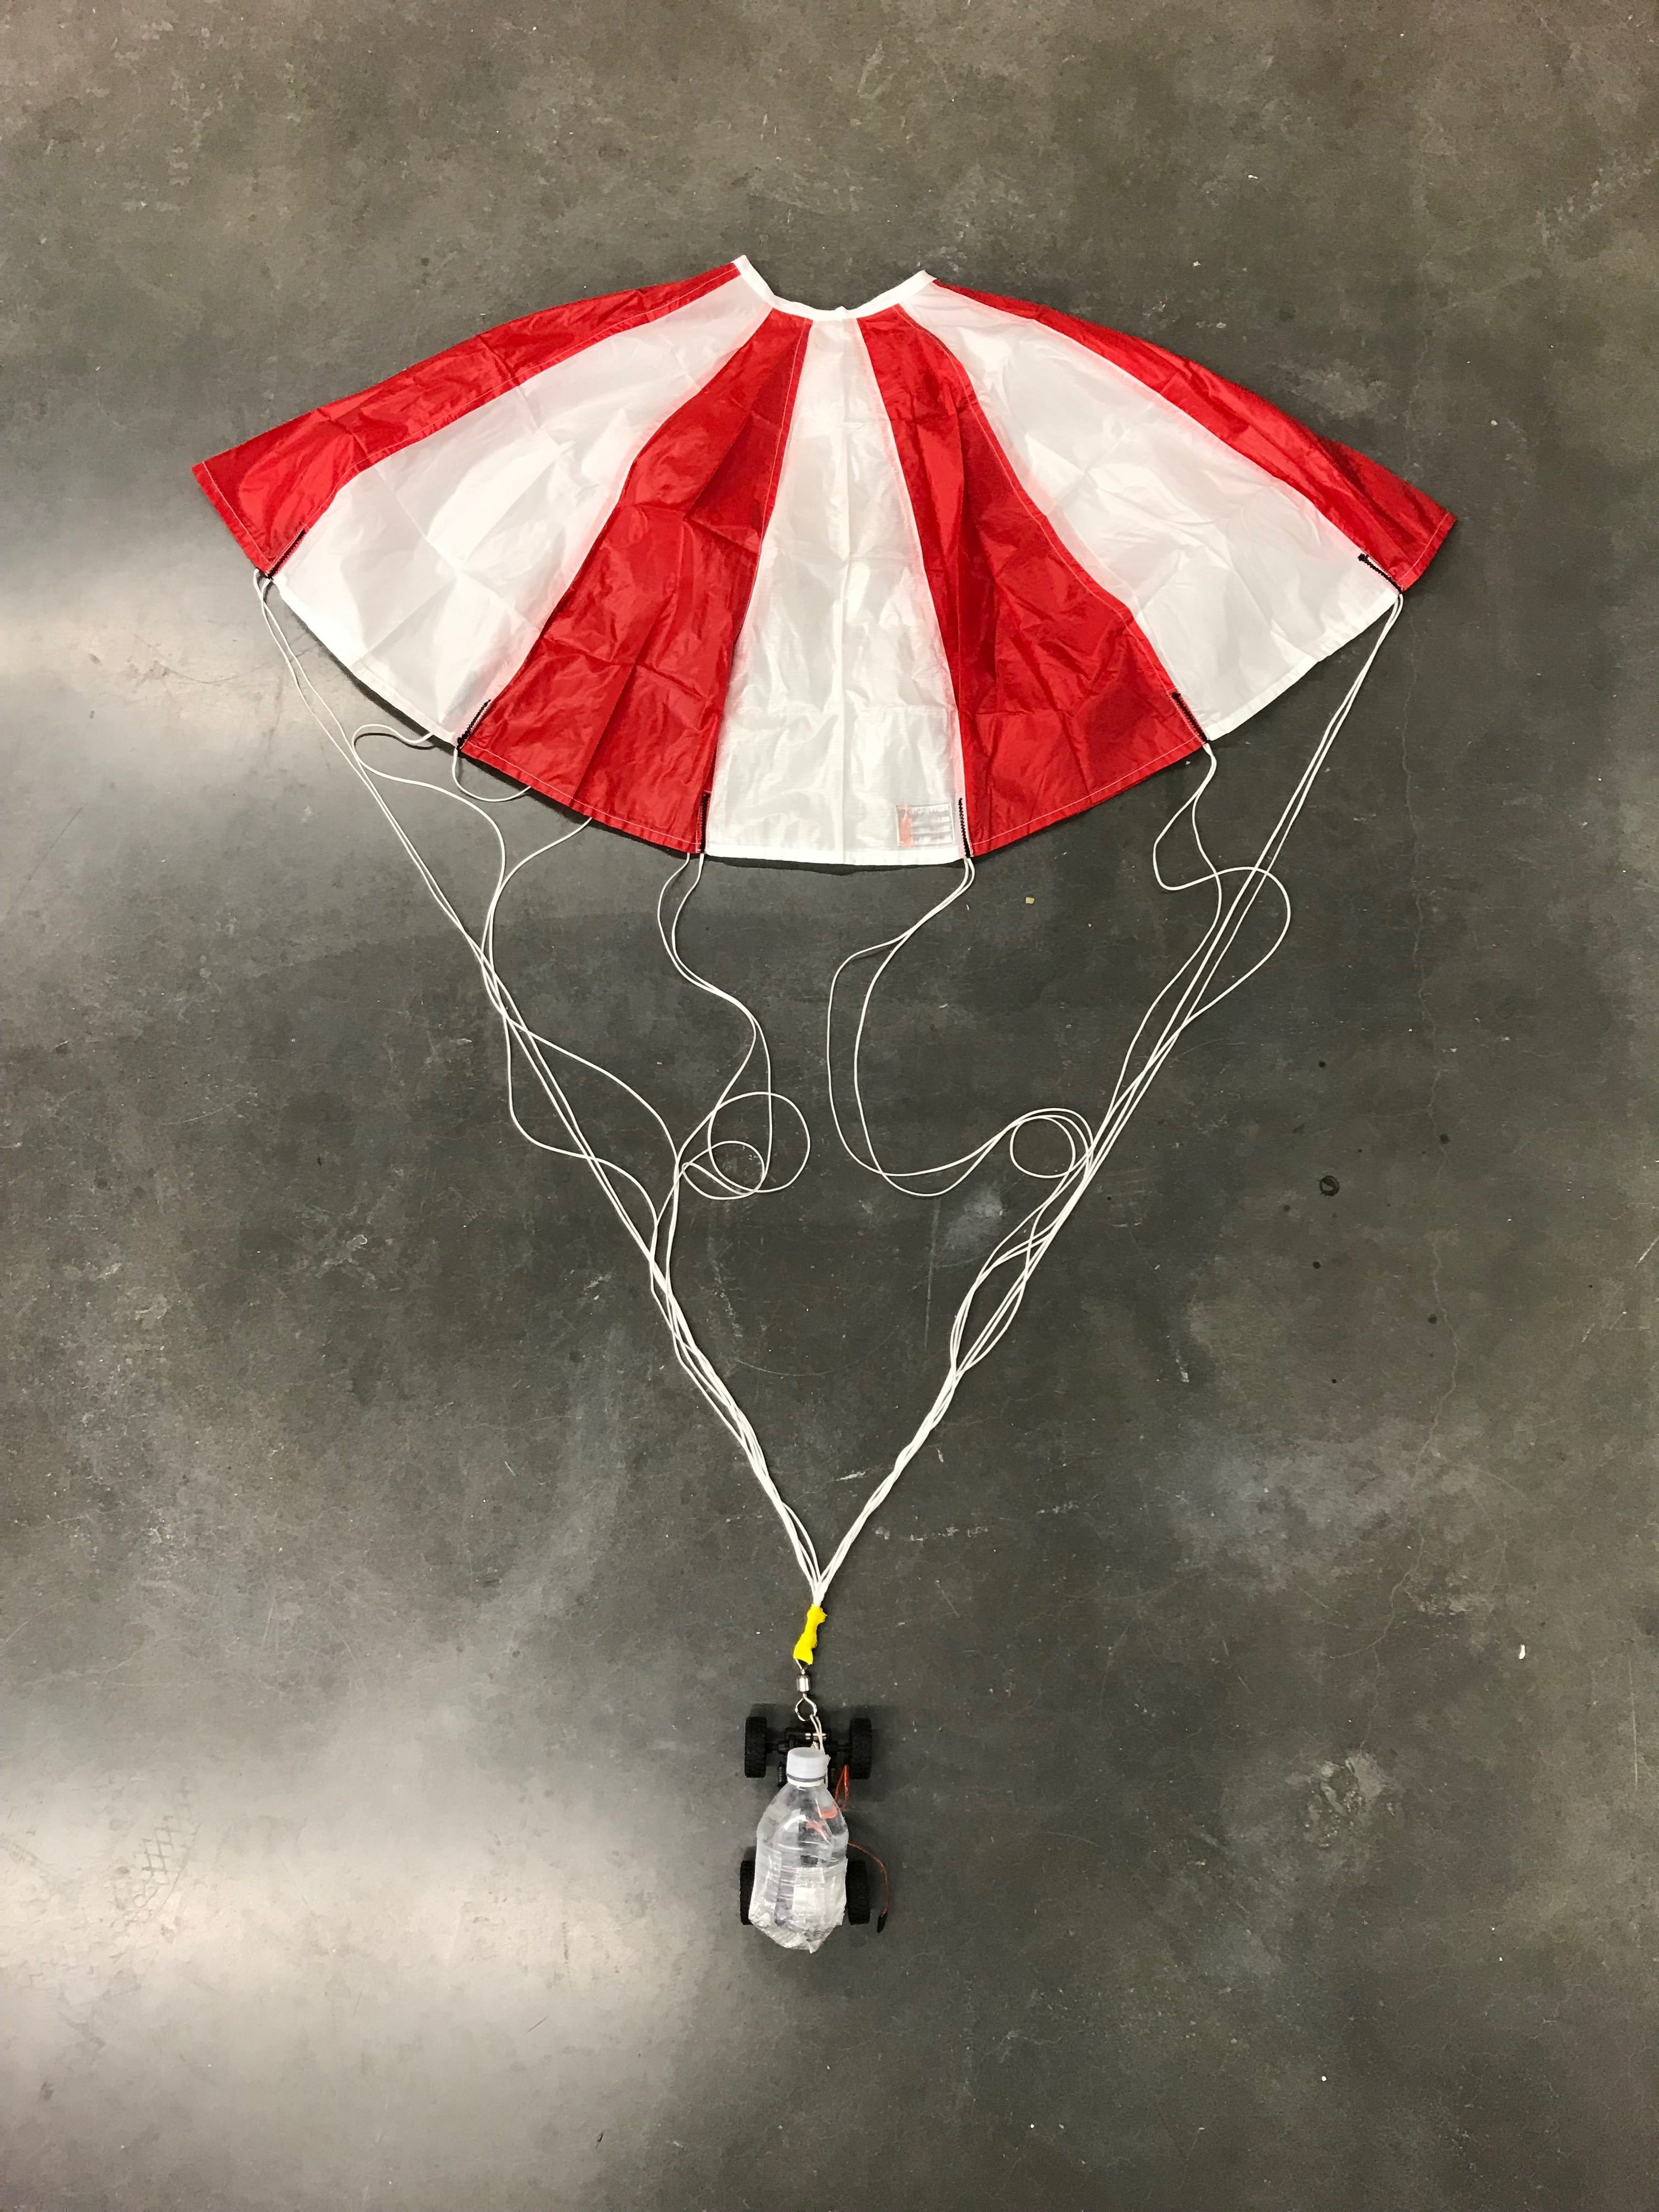
\includegraphics[width=90mm]{./figs/Parachute_Side.jpg}
\caption{Our parachute and simulated UGV as seen from the side.}
\label{fig:side}
\end{figure}

An accurate landing is an important part of the competition, and is the key success measure governing the design of the UGV drop system.
A hole in the top of the parachute improves the accuracy of the system.
This hole is known in the industry as a spill hole because it allows the air to spill out of the center of the parachute. 
This increases the velocity with which the system falls, but it also provides a marked increase in the accuracy.
This is because without the hole, the air become trapped within the system and excess air must move around the outside of the parachute as it falls.
Imperfections in manufacturing and weather conditions mean that this this overflow around the outside of the  parachute is always uneven. Thus the parachute is pushed to the side by the uneven overflow. This is analogous to pouring water into a cup. Once the cup is full, the excess water poured into it overflows over the side. A spill hole allows the overflow to "spill" out the top of the parachute in a way that won't affect the lateral velocity of the system. This is comparable to a small hole in the bottom of the analogous cup which allows the excess water to flow out the bottom of the cup instead of overflowing over the side. 

\begin{figure}[ht]
\centering
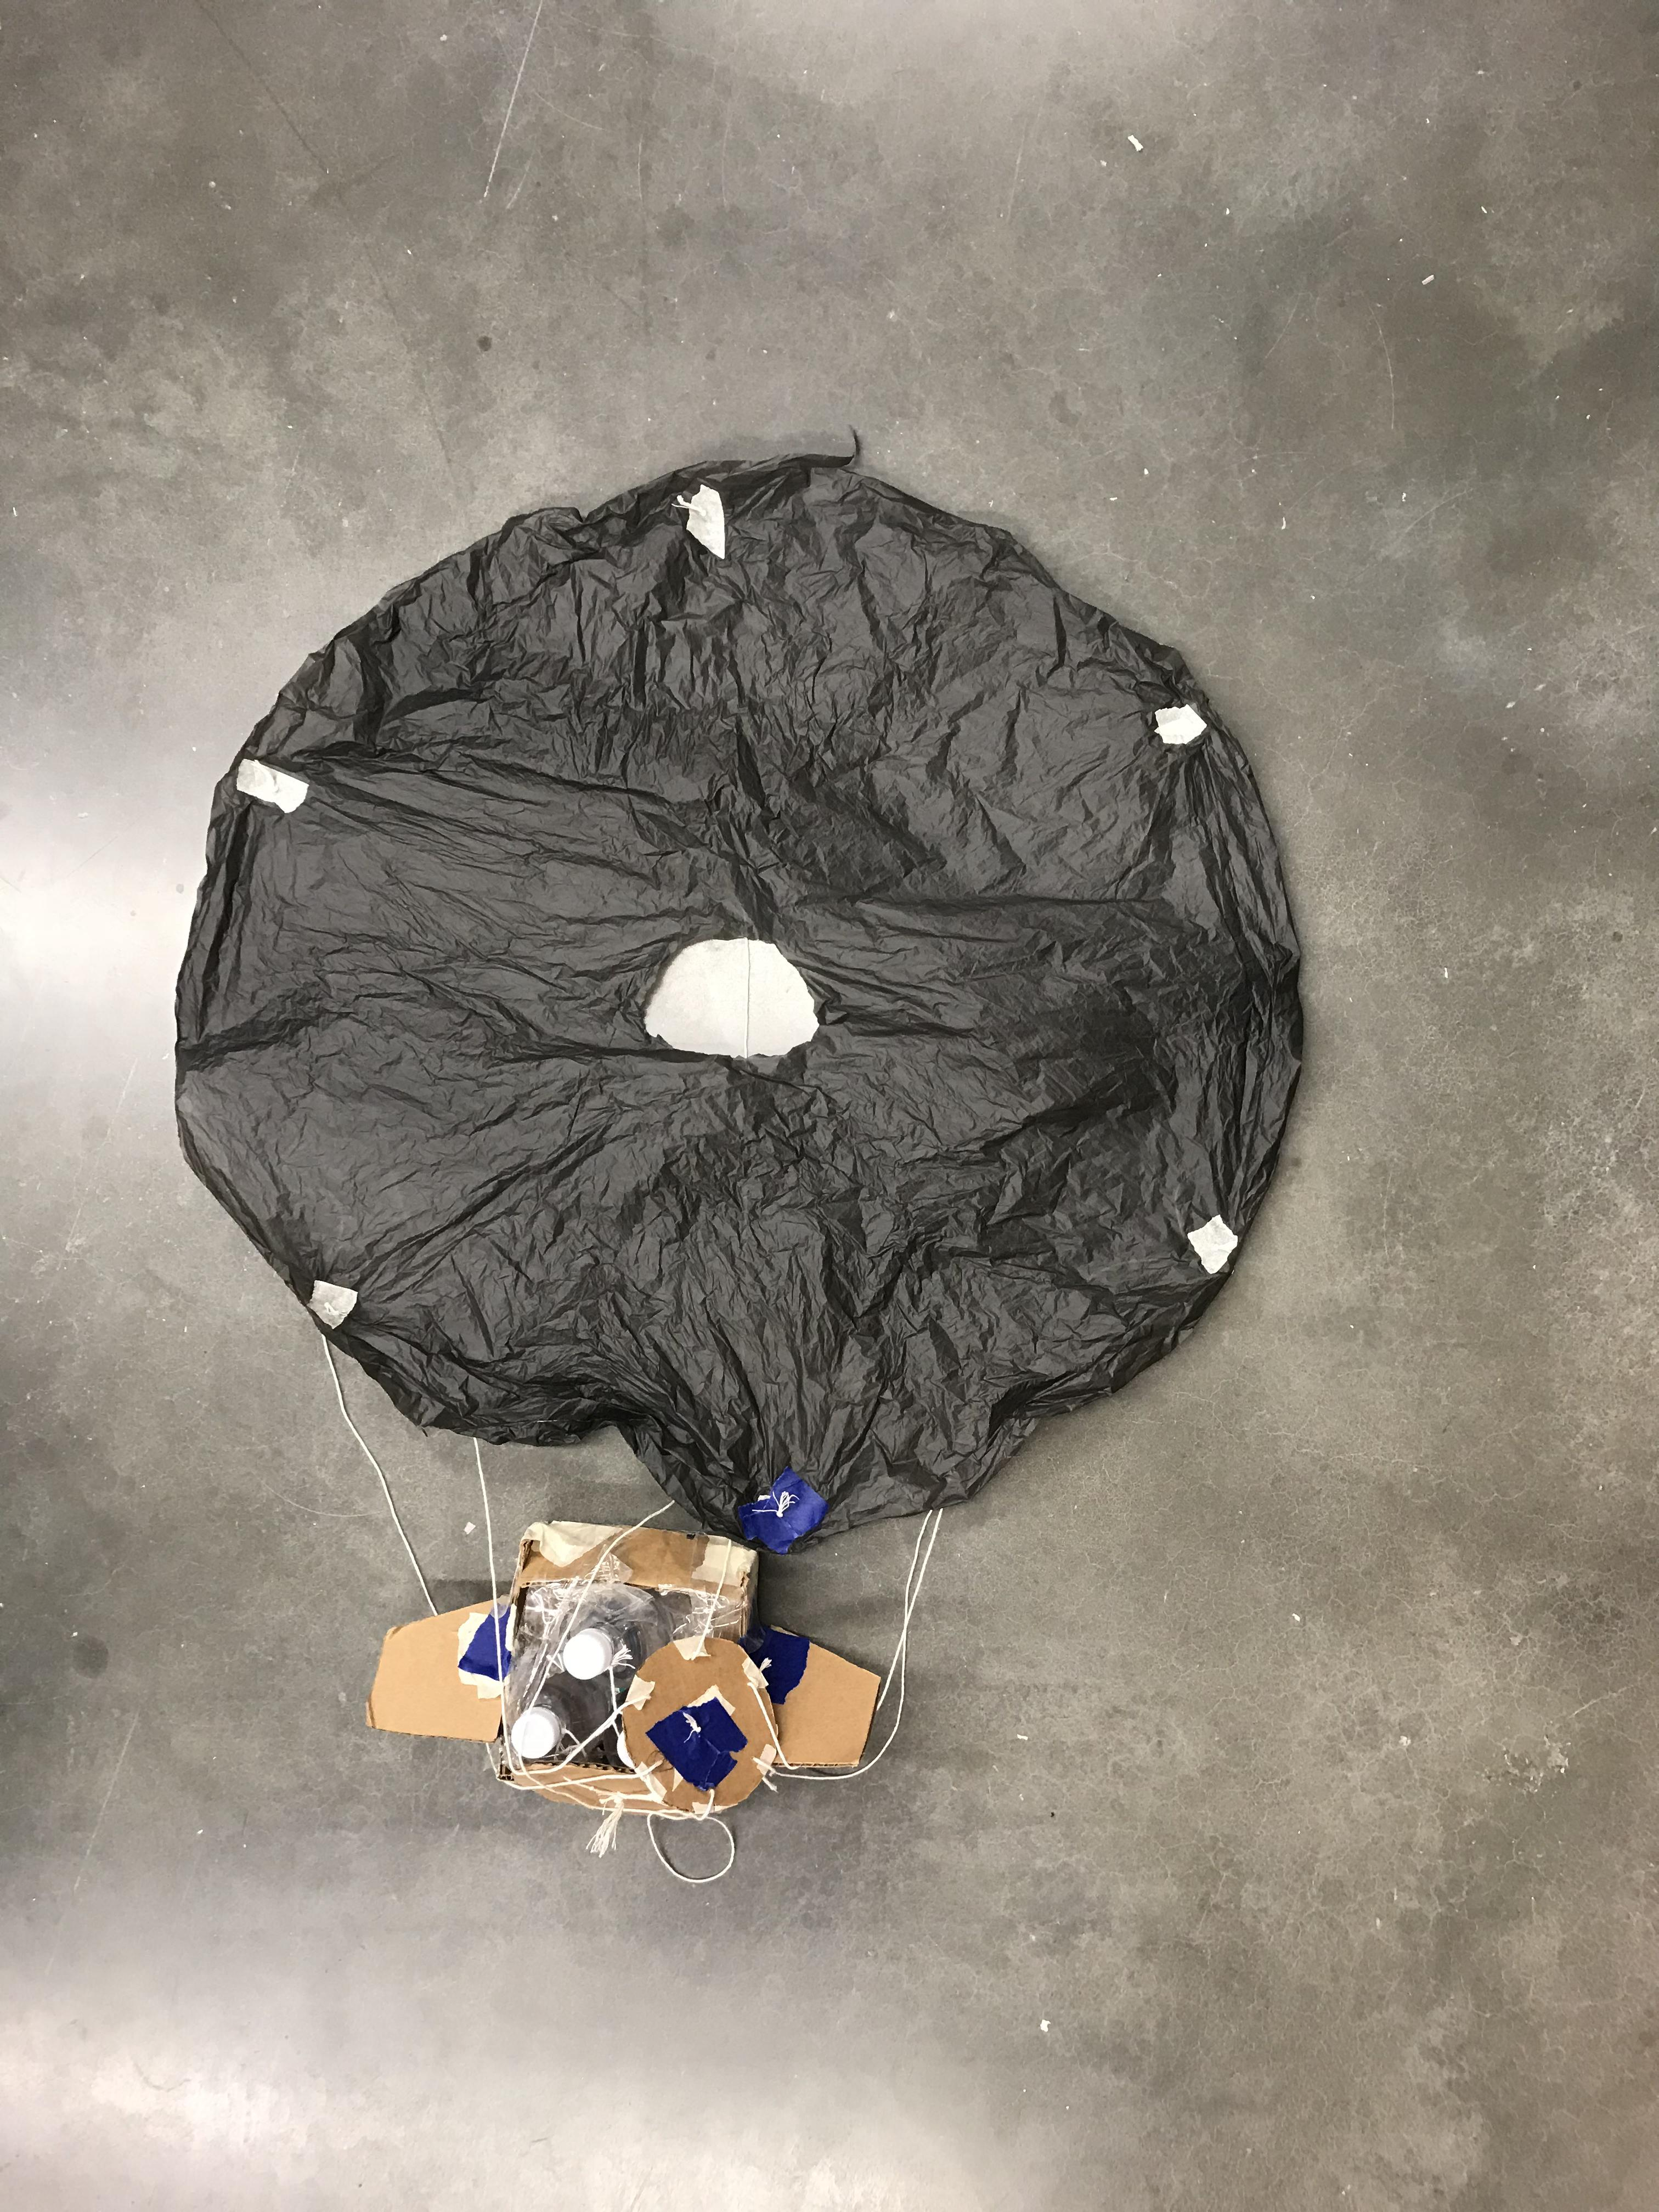
\includegraphics[width=90mm]{./figs/Parachute_Top.jpg}
\caption{A simple prototype of our parachute seen from the top. Note the hole in the middle of the parachute. As mentioned above, we found that this greatly improved the accuracy of the parachute.}
\label{fig:top}
\end{figure}

Fins are another way the accuracy of the system can be affected. These fins can be seen in our prototype in Fig.~\ref{fig:fins}. As can be seen in our testing results artifact (GV-004) the fins did push the system one direction. This should allow us to slightly control our system as it falls. While this will not be enough to correct for large errors, it should be enough to ensure the system doesn't drift randomly. The protocol for dropping objects from a UGV, as detailed in \textit{Small Unmanned Aircraft: Theory and Practice} by Randy Beard and Tim McLain, should also help improve our accuracy. This protocol uses the wind and velocity of the aircraft to predict the best location to release the payload.

\begin{figure}[ht]
\centering
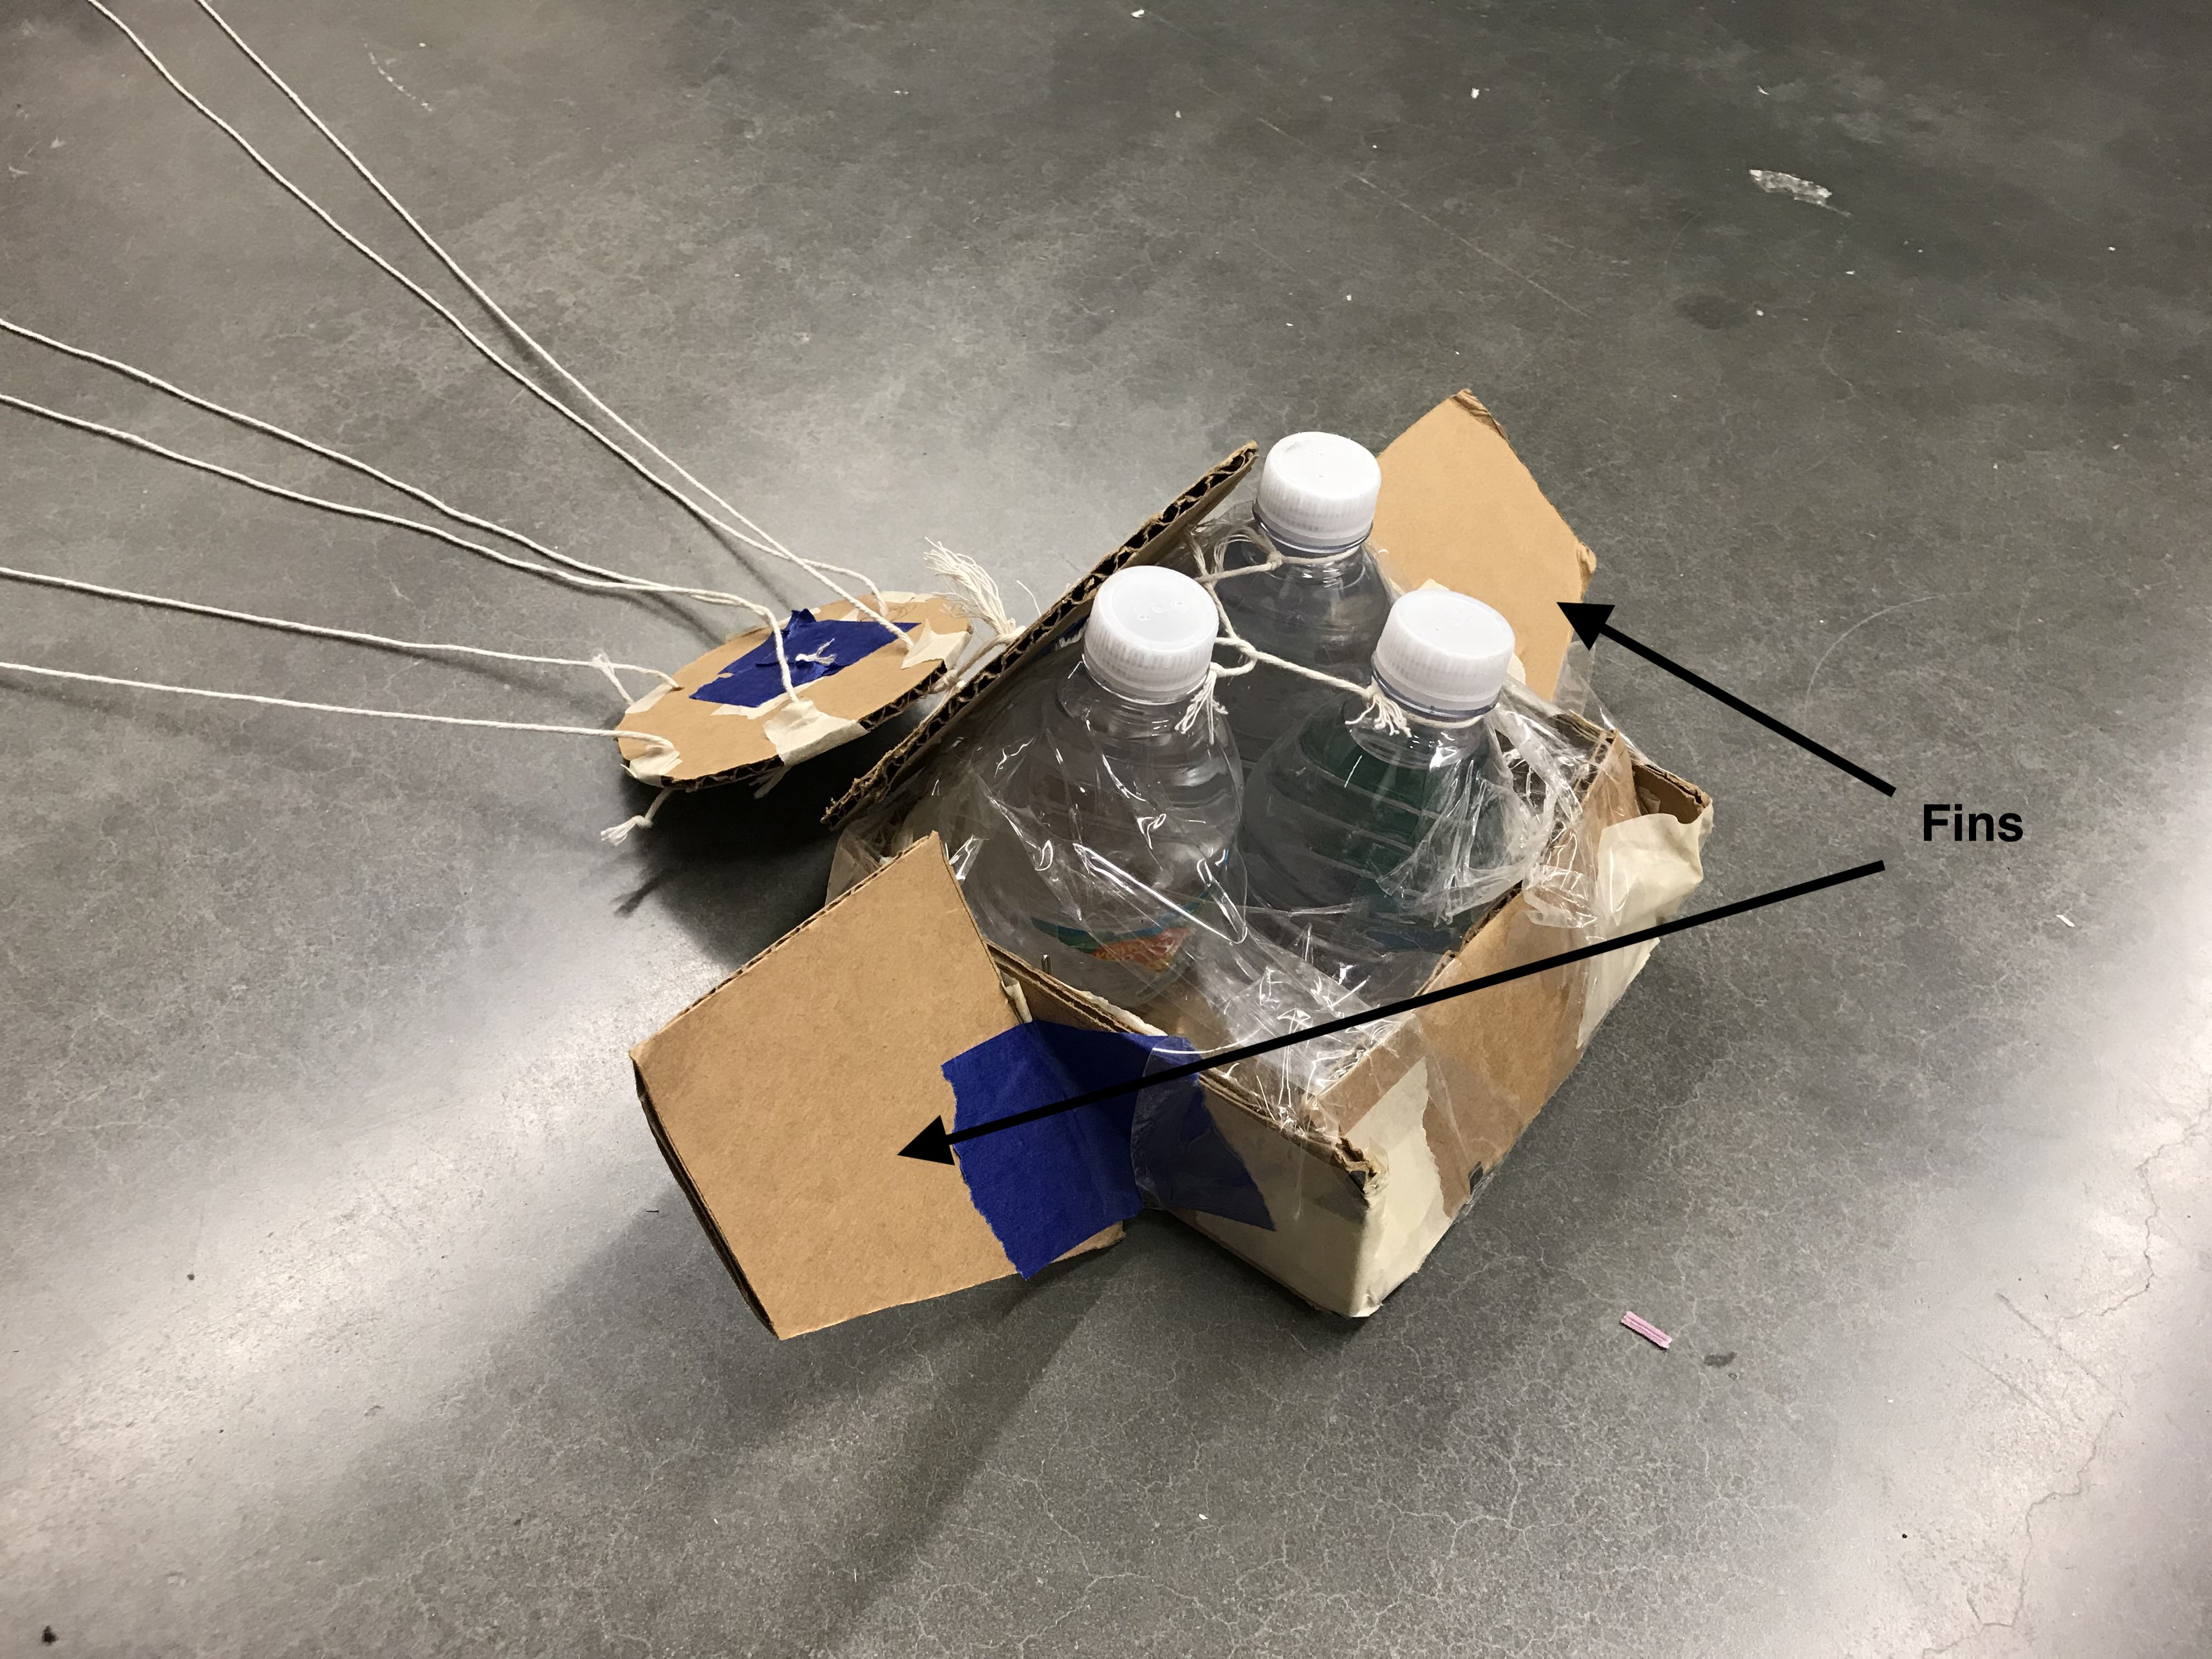
\includegraphics[width=90mm]{./figs/Parachute_Fins.jpg}
\caption{The payload we used to simulate the UGV. Note the fins. As mentioned above, preliminary results seem to indicate that these fins provided a small amount of control authority over the parachute's trajectory. This will help us improve accuracy}
\label{fig:fins}
\end{figure}

\section{Conclusion}
Using the system described above, we are confidant in our ability to achieve a landing accuracy of within 25 feet. This is considered excellent performance in our key success measures and will give us 75\% of the points possible in this portion of the competition. 

\end{document}

